\documentclass[12pt, a4paper]{article}

\usepackage[utf8]{inputenc}
\usepackage[russian]{babel}
\parindent 0pt
\parskip 8pt
\usepackage{amsmath}
\usepackage{amssymb}
\usepackage{array}
\usepackage{floatrow}
\usepackage{float}
\usepackage[left=2.3cm, right=2.3cm, top=2.7cm, bottom=2.7cm, bindingoffset=0cm]{geometry}
\usepackage{hyperref}
\usepackage{graphicx}
\usepackage{multicol}
\usepackage{listings}
\usepackage{fancyhdr} 
\usepackage{extramarks}
\usepackage[usenames,dvipsnames]{color}
\usepackage{titlesec}
\usepackage{tikz}
\usepackage[T2A]{fontenc} 
\definecolor{grey}{RGB}{128,128,128}


\title{Рабочий протокол и отчет по лабораторной работе No 5.07
\\ Определение постоянной Планка методом задерживающего потенциала
}

\author{Фадеев Артём, Елизбарашвили Серго }

\begin{document}
\maketitle

\section{Цели работы}

\begin{itemize}
    \item Экспериментально проверить законы фотоэффекта.
    \item Определение постоянной Планка и работы выхода электрона из металла.
\end{itemize}

\section{Задачи, решаемые во время выполнения работы}

\begin{itemize}
    \item Построить график зависимости энергии электронов от частоты падающего излучения, аппроксимировать полученную прямую.
    \item Определить угол наклона и частоту красной границы фотоэффекта для материала фотокатода и их погрешности.
    \item Воспользоваться справочником для определения металла, из которого сделан фотокатод.
    \item Рассчитать погрешности в измерениях постоянной Планка и работы выхода.
\end{itemize}

\section{Объект исследования}
\begin{itemize}
    \item Явление фотоэффекта.
\end{itemize}

\section{Метод эксперементального исследования}
\begin{itemize}
    \item Измерения, путём поиска оптимального значения точки нуля для разных светодиодов.
\end{itemize}

\section{Рабочие формулы и исходные данные}
\begin{itemize}
    \item $h\nu = A_{v} + \frac{m_e v^2}{2}$ -- уравнение Эйнштейна
    \item $h\nu_{0} = A_{v}$ -- работа фотоэффекта
    \item $T = eU_0$ -- условие приращения тока
    \item $U_0 = \frac{h\nu}{e} - \frac{A_{v}}{e}$ -- выражение для задерживающего напряжения
    \item $\nu = \frac{c}{\lambda}$ -- связь длины волны с частотой
    \item $\frac{\Delta h}{h} = \frac{\Delta U}{U} + \frac{\Delta \lambda}{\lambda}$ -- расчет погрешности для постоянной Планка
    \item $\frac{\Delta A}{A} = \frac{\Delta h}{h} + \frac{\Delta \nu}{\nu} = \frac{\Delta h}{h} + \frac{\Delta \lambda}{\lambda}$ -- расчет погрешности для работы выхода
\end{itemize}

\section{Измерительные приборы}
\begin{tabular}{|c|c|c|c|c| }
     \hline № & Наименование & Тип пробора  & Используемый диапазон  &Погрешность прибора \\
     \hline 1  &  Вольтметр  & цифровой & 0.07-0.7 & 1.5-2\% \\
     \hline 2 & Наноамперметр  &  цифровой  &  0-0.5  &  1.5-2\% \\
     \hline
\end{tabular}

\section{Схема установки}
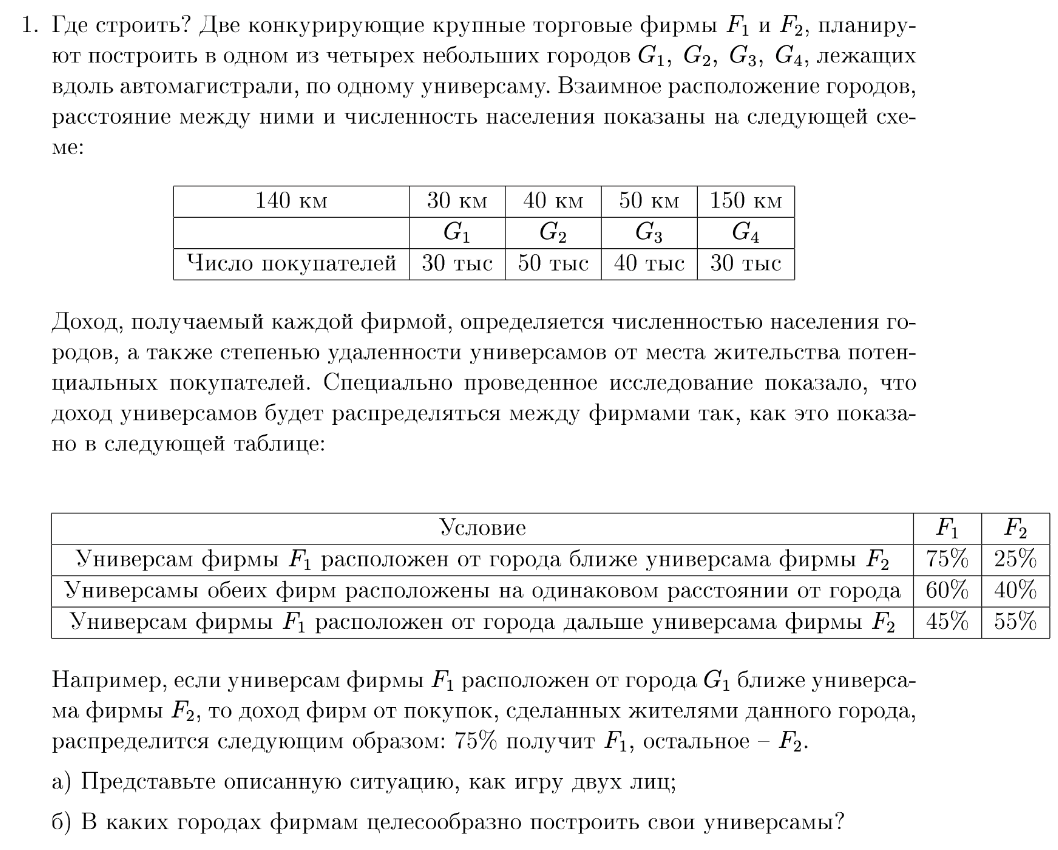
\includegraphics[]{1.png}

\section{Результаты прямых измерений и их обработки}

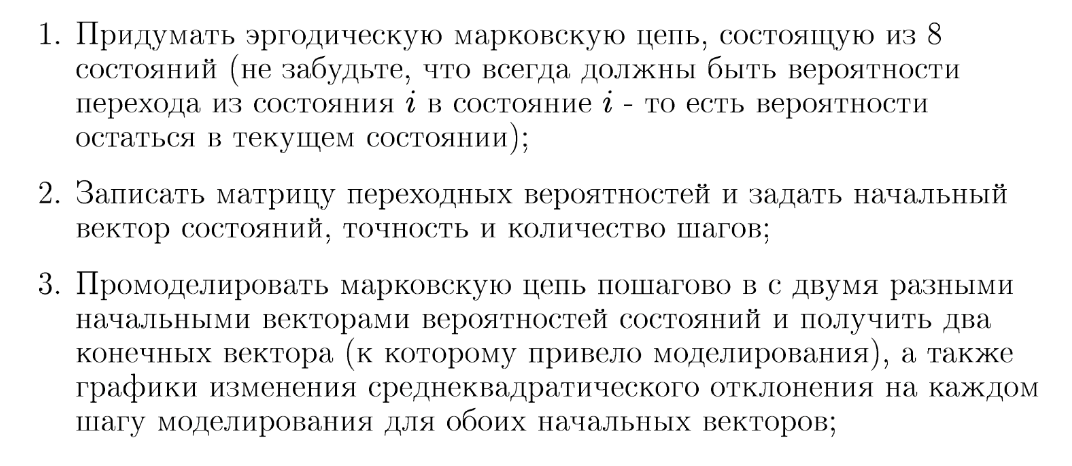
\includegraphics[]{2.png}

\section{Результаты косвенных измерений и их обработки}
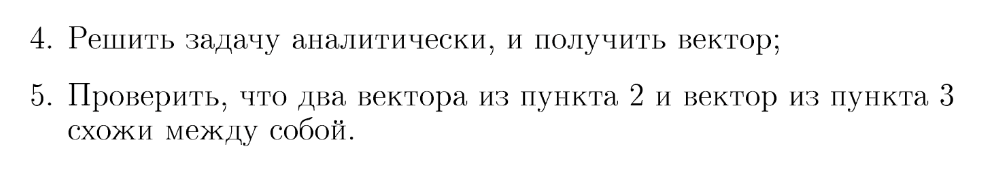
\includegraphics[]{3.png}
\newline
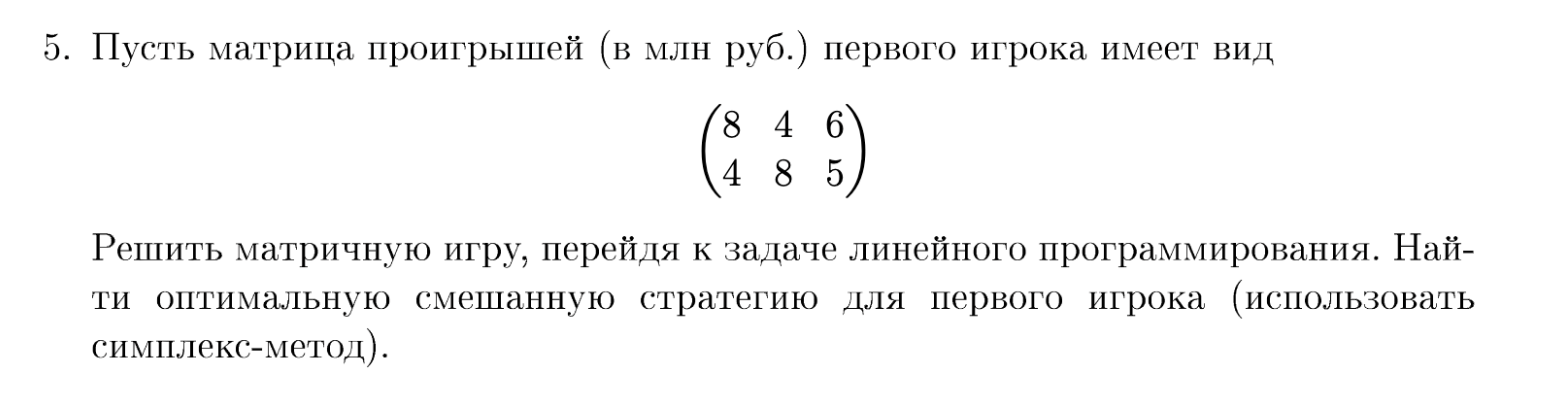
\includegraphics[]{5.png}

\item $\frac{\Delta h}{h} = \frac{\Delta U}{U} + \frac{\Delta \lambda}{\lambda} = 0.005 + 0.001 = 0.006$
    \item $\frac{\Delta A}{A} = \frac{\Delta h}{h} + \frac{\Delta \nu}{\nu} = \frac{\Delta h}{h} + \frac{\Delta \lambda}{\lambda} = 0.006 + 0.001 = 0.007$

\section{Графики}
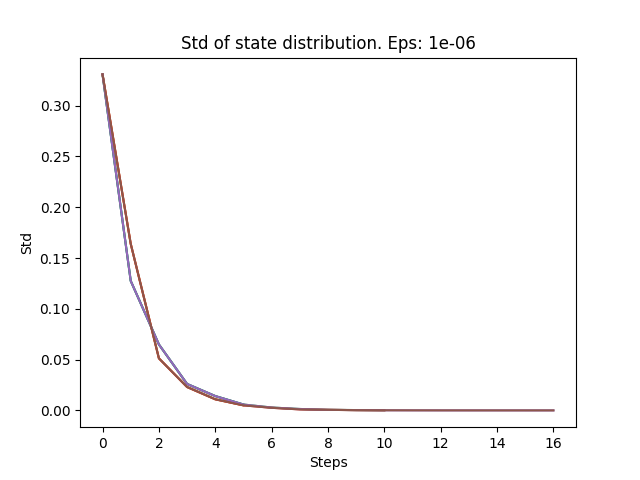
\includegraphics[]{4.png}

\section{Выводы и анализ работы}
$A_{v} = 1.904 \ eV \quad h = 6.462 \cdot 10^{-34}$
\begin{itemize}
    \item В этой лабораторной работе мы определили зависимость кинетической энергии электрона от частоты.
    \item Построив аппроксимирующую прямую, получили уравнение, позволившее определить постоянную Планка и работу выхода.
    \item Используя полученное значение работы выхода смогли определить, что материал из которого сделан фотокатод – цезий.
\end{itemize}
\end{document}
